\documentclass[../main.tex]{subfiles}

\newcommand{\kp}{k_{+}}
\newcommand{\km}{k_{-}}
\newcommand{\kz}{k_{z}}
\newcommand{\st}{S}
\newcommand{\stp}{\overline{S}_{+}}
\newcommand{\stm}{\overline{S}_{-}}
\newcommand{\swp}{\widetilde{S}_{+}}
\newcommand{\swm}{\widetilde{S}_{-}}
\newcommand{\vep}{\varepsilon}

\newcommand{\sign}{\text{sign}}


\begin{document}
    \chapter{Вычисление зонного спектра \label{chapter:calcs}}

    \section{Модель Кейна 8x8}

    \subsection{Обзор}

    В силу того, что $HgTe$ имеет отрицательную ширину запрещённой зоны,
    гетероструктуры с квантовыми ямами (КЯ) на основе $Hg_{1-x}Cd_{x}Te$ 
    могут реализовать как инвертированный, так и нормальный зонный спектр
    (например \cite{MinkovValence2017}).

    Возможность работы с чрезвычайно малыми величинами $E_g$ порядка
    $\sim 1~\mev$ налагает высокие требования на точность рассматриваемой 
    модели. Эти требования не могут быть выполнены при использовании,
    например, модели Кона-Латинджера. В то же время, как это было показано
    в \cite{Novik:2005}, \cite{Zholudev:Magnet:2012} модель Кейна 
    \cite{Kane:Band:1957} даёт воспроизводимые и близкие к экспериментальным 
    значениям результаты.

    \subsection{Однородная структура}

    В данной работе был рассмотрен гамильтониан Кейна, 
    полученный для структур, рост которых осуществаялся в 
    кристаллографическом направлении (001).

    \begin{equation}
        \hat{H} =
            \rmatrix[0.7]{
                T       &   0       & -  P \kp  /\sqrt{2}   & \sqrt{2} P \kz / \sqrt{3} & P\km /\sqrt{6}        &   0       & -P\kz /\sqrt{3}   &   -P\km / \sqrt{3}\\
                0       &   T       &   0                   &   -P\kp /\sqrt{6}         &   \sqrt{2} P\kz / \sqrt{3}    &   P\km /\sqrt{2}  &   -P\kp / \sqrt{3}    & P\kz/\sqrt{3}\\
                -\km P/\sqrt{2} & 0 & U + V & -\stm & R &   0   & \stm / \sqrt{2}   & -\sqrt{2} R\\
                \sqrt{2} \kz P  & -\km P /\sqrt{6}  &   -\stm^\dagger   & U-V   &   C   &   R   & \sqrt{2} V & -\sqrt{3} \swm /\sqrt{2}\\
                \kp P /\sqrt{6} & \sqrt{2} \kz P /\sqrt{3}  & R^\dagger & C^\dagger & U - V & \stp^\dagger  & - \sqrt{3} \swp /\sqrt{2} & - \sqrt{2} V\\
                0   &   \kp P /\sqrt{2} & 0 & R^\dagger & \stp  & U+V   & \sqrt{2} R^\dagger    & \stp/\sqrt{2}\\
                -\kz P /\sqrt{3}    & - \km P / \sqrt{3}    & \stm^\dagger /\sqrt{2}    & \sqrt{2} V    & - \sqrt{3} \stp^\dagger /\sqrt{2} & \sqrt{2} R    & U - \Delta    & C\\
                -\kp P /\sqrt{3}    & \kz P /\sqrt{3}   & - \sqrt{2} R^\dagger  & -\sqrt{3} \stm^\dagger /\sqrt{2}  & -\sqrt{2} V   & \stp^\dagger /\sqrt{2}    & C^\dagger & U - \Delta
            };
    \end{equation} 

    Этот гамильтониан подробно рассмотрен в статье \cite{Novik:2005}.
    Вид каждого отдельного элемента может быть найден в этой же статье. Важно лишь
    отметить, возможность представления такого элемента как билинейной формы:
    \begin{equation}
        Q = (1,k_x,k_y,k_z) \cdot \hat{Q}_{4 \times 4} \cdot (1,k_x,k_y,k_z)^{T};
    \end{equation}
    В дальнейшем это позволит более просто вычислять матричные элементы для состояний
    с разными значениями волновых векторов.


    Этот гамильтониан действует в пространстве комплексных векторов размерности $8 \times 1$,
    описывающих разложение по Блоховским функциям:

    \begin{equation*}
        \psi_i(\vec r) = c_i \exp(i \vec k \vec r) u_i (\vec r);
    \end{equation*}

    Требуется отметить, что этот гамильтониан приведён для объёмного материала.
    В силу того, что в данной работе рассматриваются гетероструктуры состав 
    $Hg_{1-x}Cd_{x}Te$ оказывается сильно неоднородным по оси $\vec{z}_0$.

    \subsection{Случай гетероструктуры}

    Для начала стоит обсудить проблему выбора базиса. В силу того, что нас 
    интересуют состояния, локализованные внутри квантовых ям мы можем выбрать
    для рассмотрения конечный по оси $\vec{z}_0$ участок гетероструктуры длиной
    $L$. Это возможно для $L \gg d \exp(- E_ь / E_{g, bar})$ ($d$ - толщина квантовой
    ямы, $E_ь$ - разница энергии $ь$-ого уровня в $\Gamma$ точке, $E_{g,bar}$ - 
    ширина запрещённой зоны в однородном материале барьера).

    Базисными функциями по оси $\vec{z}_0$ выберем плоские волны 
    $\frac{1}{\sqrt L} \exp(i k_{z,m} z)$, c квантованным значением проекции 
    квазиимпульса: 
    
    \begin{equation}
        \label{k_vec}
        k_{z,m} = \frac{2\pi}{L} m;
    \end{equation}

    В таком случае, при фиксированном $\vec{k}_\perp = (k_x,k_y)$ базисные 
    функции имеют два индекса: отвечающий Блоховской функции $i$, уровню размерного
    квантования $m$ для бесконечной ямы ширины $L$. Базисная функция:

    \begin{equation}
        \psi_{i,m}(\vec r) = c_{i, m} \exp(i \vec{k}_\perp \vec{r}_\perp) \exp(i k_{z,m} z) u_i(\vec r);
    \end{equation}

    Полная волновая функция будет иметь вид:
    \begin{equation}
        \label{calculation:wf}
        \Psi = \sum_m \exp(i \vec{k}_{m} \vec r) \sum_{i}  c_{i,m} u_i(\vec r);
    \end{equation}
    Где $\vec{k}_m = (\vec{k}_\perp,k_{z,m})$ - волновой вектор, с учётом (\ref{k_vec}). 

    Тогда мы можем перейти в представление, связанное с коэффициентами $c_{i,m}$. 
    Будем группировать эти коэффициенты в "вектора", отвечающие одному уровню 
    размерного квантования:
    \begin{equation*}
        \vec{c}_m = (c_{0, m},\hdots,c_{7, m});
    \end{equation*}

    Также для перехода в такое представление нам потребуется перейти к операторам,
    при записи каждого элемента "объёмного" гамильтониана Кейна: 
    $H_{i,j} \rightarrow \hat{H}_{i,j}$. Это можно сделать, вычислив матричные 
    значения на огибающих функциях:
    \begin{equation}
        \hat{H}_{(i, j)(m, s)} = \frac{1}{l} \int_0^L \exp(- i k_{z, m} z) H_{i,j}(z)
            \exp(i k_{z, s} z) dz;
    \end{equation}

    Гамильтониан Кейна в таком случае примет блочный вид и запишется как:
    \begin{equation}
        \hat H = \{\hat{H}_{m, s}\}
    \end{equation}

    Дальнейшее решение задачи сводится к диагонализации полученной матрицы при 
    каждом конкретном $\vec{k}_\perp$ или, говоря иначе, к разложению:
    \begin{equation*}
        \hat H = Q^{\dagger} \Lambda Q;
    \end{equation*}
     
    В таком случае $\Lambda$ - диагональная матрица с уровнями энергии, а $Q$ - 
    матрица собственных векторов или коэффициентов разложений волновых функций.


    \section{Гамильтониан напряжений}

    \subsection{Учёт напряжения}
    Задача учёта механического напряжения является акутальной для данных материалов, 
    поскольку величины ширины запрещённой зоны могут быть сопоставимыми таки
    с энергией механического напряжения.

    Такой учёт может быть произведён в том же формализме, добавляя к гамильтониану 
    Кейна некий эффективный гамильтониан напряжений:
    \begin{equation}
        \hat{H}_\epsilon =
            \rmatrix[0.7]{
                T_\epsilon       &  0 & 0 & 0 & 0 & 0 & 0 & 0\\
                0    &   T_\epsilon   & 0 & 0 & 0 & 0 & 0 & 0\\
                0    & 0  & U_\epsilon + V_\epsilon         & -\st_\epsilon                             & R_\epsilon                                & 0                              & \st_\epsilon / \sqrt{2}           & -\sqrt{2} R_\epsilon\\
                0    & 0  & -\st^\dagger_\epsilon           & U_\epsilon - V_\epsilon                   & 0                                         & R_\epsilon                     & \sqrt{2} V_\epsilon               & -\sqrt{3} \st_\epsilon /\sqrt{2}\\
                0    & 0  & R^\dagger_\epsilon              & 0                                         & U_\epsilon - V_\epsilon                   & \st^\dagger_\epsilon           & - \sqrt{3} \st_\epsilon /\sqrt{2} & - \sqrt{2} V_\epsilon\\
                0    & 0  & 0                               & R^\dagger_\epsilon                        & \st_\epsilon                              & U_\epsilon+V_\epsilon          & \sqrt{2} R_\epsilon^\dagger       & \st_\epsilon/\sqrt{2}\\
                0    & 0  & \st^\dagger_\epsilon /\sqrt{2}  & \sqrt{2} V_\epsilon                       & - \sqrt{3} \st^\dagger_\epsilon /\sqrt{2} & \sqrt{2} R_\epsilon            & U_\epsilon - \Delta_\epsilon      & 0\\
                0    & 0  & - \sqrt{2} R^\dagger_\epsilon   & -\sqrt{3} \st^\dagger_\epsilon /\sqrt{2}  & -\sqrt{2} V_\epsilon                      & \st^\dagger_\epsilon /\sqrt{2} & 0                                 & U_\epsilon - \Delta_\epsilon
            };
    \end{equation} 

    Элементы этого гамильтониана также приведены в работе \cite{Novik:2005} и зависят 
    лишь от тензора деформации в точке $\vep_{ij}(z)$.

    \subsection{Расчёт напряжения}

    В практических применениях часто используется т.н. "приближение тонкой плёнки":
    считается, что, если "тонкая" гетероструктура c параметром решётки $a(x)$ выращенна 
    на "толстом" слое материала с параметром решётки $\alpha_0$, то она будет "наследовать"
    его. Вообще говоря это характерно для плёнок с толщиной $l$, выращенных на буффере, 
    толщиной $L$ такой, что выполняется: $l / L \ll (a - a_0) / a_0$.

    В нашем случае это приближение является справедливым, так как 
    $L \sim 10 \mu m,~l \sim 10 nm$, a $(a - a_0) / a_0 \sim 1 / 20$. 

    Таким образом, поскольку мы рассматриваем тонкую плёнку, то мы знаем
    некоторые компоненты тензора деформация:
    \begin{equation}
        \label{well_known_components}
        \vep_{xx}(z) = \vep_{yy}(z) = \frac{a(z) - a_0}{a_0},~\vep_{xy} = \vep_{yx} = 0;
    \end{equation}

    Задача сводится к отысканию $\vep_{zz},\vep_{xz},\vep_{yz}$. 
    Можно воспользоваться законом Гука, связывающего тензор натяжений 
    и тензор деформаций (вид тензора $C_{ijkl}$ можно увидеть в \cite{Landau:Upr:1965}):
    \begin{equation}
        \label{gook_law}
        \sigma_{ij}(z) = \sum_{k,l} C_{ikjl}(z) \vep_{k,l}(z);
    \end{equation}

    Вообще говоря, тензор натяжений в равновесии связан с внешними силами как:
    \begin{equation}
        \sum_j \frac{\partial \sigma_{ij}(z)}{\partial x_j} + F_i(z) = 0;
    \end{equation}

    В нашем случае плоскослоистой среды без внешних сил это приводит к условию:
    $\sigma_{iz} = 0$. А сама задача сводится к решению простой системы линейных
    уравнений в каждой точке по оси z:
    \begin{equation}
        \sum_k C_{ikzk} \vep_{kz} + (C_{ixzx} \vep_{xx} + C_{iyzy} \vep_{yy})  = 
            \sigma_{iz} = 0, ~\forall i;
    \end{equation}

    \section{Случай отличного от (001) направления роста структур}

    В силу целого ряда технологических причин направление роста (001)
    не является оптимальным для подобных структур. Гораздо более выгодным оказываются
    направления (013), (011). Они характеризуются большей скоростью роста 
    и более низкой концентрацией дефектов.

    Таким образом встаёт задача расчёта энергетического спектра для подобных структур.

    \subsection{Гамильтониан Кейна}

    Рассмотрим некое направление роста (hkl) и найдём углы Эйлера, на которые он повёрнут
    относительно <<эталонного>> направления (001).

    \begin{eqnarray}
        \phi(\alpha) = \atan \frac{\sin \alpha}{\cos \alpha} + 
            \left\{ \begin{aligned}
                        &0 & \cos \alpha > 0;\\
                        &\sign(\sin \alpha) & \cos \alpha < 0;
                    \end{aligned}\right.;\\
        (x, y, z) = (h, k, l) / \sqrt{h^2 + k^2 + l2^2};\\
        \begin{aligned}
            &\sin \alpha  = z, & \cos \alpha = \sqrt{1 - z^2};\\
            &\sin \beta  = y
        \end{aligned}
    \end{eqnarray}

    Тогда мы могли бы перейти в нашем рассмотрении от неизвестного гамильтониана Кейна
    для структур, выращенных в направлении (hkl), к уже известным. Введём две системы 
    координат $K,~K'$, повёрнутые друг относительно друга на вышупомянутые углы Эйлера. 

    Переходу из одной системы в другую соответствует применение к вектору
    $\vec r$ матрицы вида:
    \begin{equation}
        \hat K =
        \underbrace{
            \begin{bmatrix}
                \cos \alpha & -\sin \alpha  &   0\\
                \sin \alpha & \cos \alpha   &   0\\
                0           & 0             &   1
            \end{bmatrix}
        }_{\hat{K}_z(\alpha)}
        \underbrace{
            \begin{bmatrix}
                \cos \beta  & 0             &   \sin \beta \\
                0           & 1             &   0\\
                -\sin \beta & 0             &   \cos \beta
            \end{bmatrix}
        }_{\hat{K}_y(\beta)}
        \underbrace{
            \begin{bmatrix}
                \cos \gamma & -\sin \gamma  &   0\\
                \sin \gamma & \cos \gamma   &   0\\
                0           & 0             &   1
            \end{bmatrix}
        }_{\hat{K}_z(\gamma)}
    \end{equation}

    Аналогично преобразуется и волновой вектор $\vec k$. В то же время требуется изменить и 
    гамильтониан. Сам гамильтониан опредлён, как матричные элементы, между волновыми функциями,
    являющимися собственными для оператора момента импульса по оси z (здесь $\langle \hat H \rangle$
    - матрица оператора):
    \begin{equation*}
        \bra{1} \hat H \ket{2} = \sum_{i,j} C^{(1) *}_i \bra{u_i} \hat H \ket{u_j} C^{(2)}_j
            = \vec{C}^{(1) \dagger} \langle \hat H \rangle \vec{C}^{(2)};
    \end{equation*}

    Соответственно наша задача сводится к отысканию матрицы преобразования $\hat R$,
    связывающей коэффициенты разложения в при разных поворотах:
    \begin{equation*}
        \hat R \vec{C} = \vec{C}';
    \end{equation*}

    Эта матрица является сопряжённой $\hat R = \hat T ^{*}$ к оператору поворота вектора
    базисных функций:
    \begin{equation*}
        \hat T \vec{u} = \vec{u}';
    \end{equation*}

    При этом обычно матрица поворота гамильтониана вводится как:
    \begin{equation}
        \hat R = \exp(i\hat{J}_z \gamma) \exp(i\hat{J}_y \beta) \exp(i\hat{J}_x \alpha);
    \end{equation}

    Здесь $\hat{J}_i,~i = x, y, z$ - операторы проекции полного момента импульса на соответствующие
    координаты.

    \subsection{Гамильтониан деформации}

    Тензор деформации при повороте меняется как (из \cite{Landau:Upr:1965}):
    \begin{equation}
        \hat{\varepsilon}^{'} = \hat{R} \hat{\varepsilon} \hat{R}^T;
    \end{equation}
    Однако это не единственное изменения, требуемое для корректного учёта смены системы координат.

    В силу поворота системы координат тензор модулей упругости $\hat C$, связывающая тензор напряжений $\hat \sigma$ 
    с тензором деформации $\hat \varepsilon$ также изменится при повороте системы координат.

    В таком случае получаем:
    \begin{equation}
        \label{transform_sigma_vep}
        \begin{aligned}
            \hat{\vep}^{'}_{ij} = \hat{R}_{ik} \hat{R}_{jl} \hat{\vep}_{kl};\\
            \hat{\sigma}^{'}_{ij} = \hat{R}_{ik} \hat{R}_{jl} \hat{\sigma}_{kl};  
        \end{aligned}
    \end{equation}

    Это удобно переписать при помощи прямого матричного умножения:
    \begin{equation*}
        \hat{\mathbb{R}} = \hat R \otimes \hat R;
    \end{equation*}

    То есть если расписывать покомпонентно: 
    \begin{equation*}
        \hat{\mathbb{R}}_{ijkl} = \hat{R}_{ij} \hat{R}_{kl};
    \end{equation*}

    Для работы удобно ввести 6-и и 9-и компонентные вектора вместо настоящих тензоров
    (введение так называемой нотации Фойгта \cite{Aquis:Tensor:2011}):

    \begin{equation}
        \hat \varepsilon 
        \equiv
        \begin{bmatrix} 
            \vep_{xx} & \vep_{yx} & \vep_{zx}\\
            \vep_{xy} & \vep_{yy} & \vep_{zy}\\
            \vep_{xz} & \vep_{yz} & \vep_{zz}
        \end{bmatrix}
        \rightarrow
        \varepsilon_{6}
        \equiv
        \begin{bmatrix}
            \vep_{xx}\\
            \vep_{xy}\\
            \vep_{yy}\\
            \vep_{xz}\\
            \vep_{yz}\\
            \vep_{zz}
        \end{bmatrix}
        \rightarrow
        \varepsilon_{9}
        \equiv
        \begin{bmatrix}
            \vep_{xx}\\
            \vep_{xy}\\
            \vep_{xz}\\
            \vep_{yx}\\
            \vep_{yy}\\
            \vep_{yz}\\
            \vep_{zx}\\
            \vep_{zy}\\
            \vep_{zz}
        \end{bmatrix};
    \end{equation}
    И аналогично преобразование в вектор и тензора напряжений $\sigma$, соответственно тензор модулей упругости может быть превращён в матрицу $6 \times 6$.
    При этом между этими матрицами существуют преобразования: $\hat{T}_{6\rightarrow 9}, \hat{T}_{9\rightarrow 6}$. Эти матрицы взаимно обратны.

    В таком случае можно написать закон Гука (\ref{gook_law}) в изначальной системе координат, 
    но другой форме:
    \begin{equation}
        \hat{T}_{9 \rightarrow 6} \hat{\sigma}_{9} = \hat{\sigma}_{6} = \hat{C} \hat{\sigma}_{6} = \hat{C} \hat{T}_{9 \rightarrow 6} \hat{\vep}_{9};
    \end{equation}

    В таком случае при непосредственно повороте у нас по известному закону преобразуются тензоры деформации и напряжений (\ref{transform_sigma_vep}) и мы сможем
    получить закон преобразования тензора $\hat{C}$:
    \begin{equation*}
        \hat{T}_{9 \rightarrow 6} \hat{\mathbb{R}}^\dagger \hat{\sigma}^{'}_{9} = \hat{C} T_{9 \rightarrow 6} \hat{\mathbb{R}}^\dagger \hat{\vep}^{'}_{9};
    \end{equation*}

    Или возвращаясь к работе с 6-и мерными векторами:
    \begin{equation}
        \hat{T}_{9 \rightarrow 6} \hat{\mathbb{R}}^\dagger \hat{T}_{6 \rightarrow 9} \hat{\sigma}^{'}_{6} = \hat{C} T_{9 \rightarrow 6} \hat{\mathbb{R}}^\dagger \hat{T}_{6 \rightarrow 9} \hat{\vep}^{'}_{6};
    \end{equation}

    Пользуясь ранее обсуждёнными свойствами матриц и определением ${\hat{\sigma}_6^{'} = \hat{C}^{'} \hat{\vep}_6^{'}}$:
    \begin{equation}
        \label{tensor_uprugosty_povorot}
        \hat{C}^{'} =  \big(\hat{T}_{9 \rightarrow 6} \hat{\mathbb{R}} \hat{T}_{6 \rightarrow 9}\big) \hat{C} \big(\hat{T}_{9 \rightarrow 6} \hat{\mathbb{R}}^\dagger \hat{T}_{6 \rightarrow 9}\big);
    \end{equation}



    Таким образом задача получения модифицированного гамильтониана сводится к:

    \begin{itemize}
        \item Вычислению $\vep_{xx}^{'},~\vep_{xy}^{'},~\vep_{yy}^{'}$ как обычно (\ref{well_known_components}).
        \item Получению тензора модулей упругости по формуле (\ref{tensor_uprugosty_povorot}).
        \item Получению оставшихся тензоров деформации.
    \end{itemize}

    В остальном процедура полностью аналогична работе с Гамильтонианом Кейна.

    Программно это может быть реализовано в виде решения вышеописанной задачи в некотором небольшом наборе точек и дальнейшей аппрокимации результатов сплайнами для улучшения производительности.


    \subsection{Результаты численных экспериментов}

    Было решено для демонастрации произвести расчёты для двух структур №170130
    (Рис. \ref{sample_170130_spectrum}) и №190225 (Рис. \ref{sample_190225_spectrum}). 
    Эти структуры были подробно описаны в частности в работе \cite{MineNanophysics2020}.

    \begin{figure}[h]
        \begin{minipage}[h]{0.49\textwidth}
            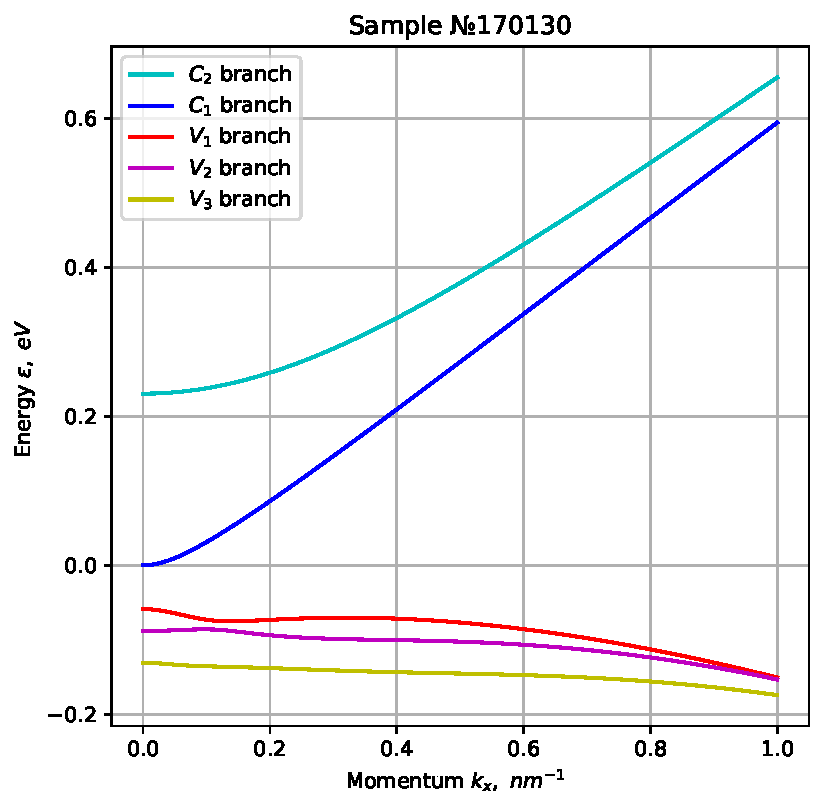
\includegraphics[width=0.9\textwidth]{./images/sample_170130_013.pdf}
            \caption{Срез дисперсионных соотношений для структуры №170130 в плоскости $k_y = 0$. \label{sample_170130_spectrum}}
        \end{minipage}
        \hfill
        \begin{minipage}[h]{0.49\textwidth}
            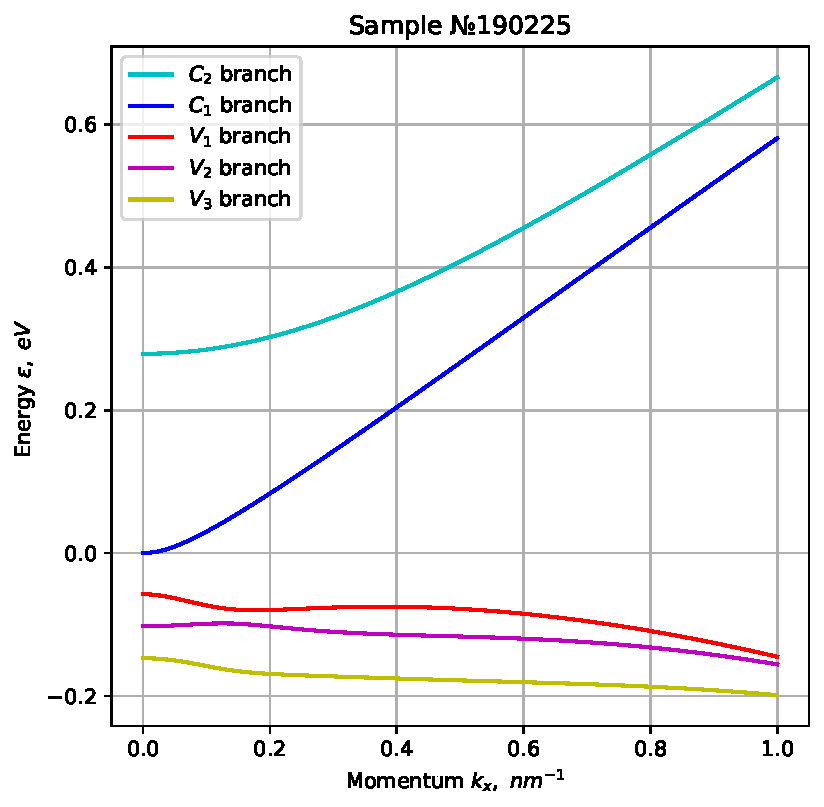
\includegraphics[width=0.9\textwidth]{./images/sample_190225_013.pdf}
            \caption{Срез дисперсионных соотношений для структуры №190225 в плоскости $k_y = 0$. \label{sample_190225_spectrum}}
        \end{minipage}
    \end{figure}

    Эти результаты хорошо согласуются с ранее полученными.

\end{document}